\documentclass[../main.tex]{subfiles}

\begin{document}

\section{NeuroCausal: Development of an Open Source Platform for the Storage, Sharing, Synthesis, and Meta-Analysis of Neuropsychological Data} 

\authors{Isil Poyraz Bilgin\textsuperscript{1}, Francois Paugam\textsuperscript{2},  Ruoqi Huang\textsuperscript{3}, Ana Luísa Pinho\textsuperscript{4, 5}, Yuchen Zhou\textsuperscript{6}, Sladjana Lukic\textsuperscript{7}, Pedro Pinheiro-Chagas\textsuperscript{8}, Valentina Borghesani\textsuperscript{9}}

\affiliations{1. Centre de recherche de l'Institut universitaire de gériatrie de Montréal, University of Montreal, Canada, 2.
University of Montreal, Montreal, Quebec, Canada, 3. University of Toronto, Toronto, Ontario, Canada, 4. Western Institute for Neuroscience, Western University, London, Ontario, Canada, 5. Department of Computer Science, Faculty of Science, Western University, London, Ontario, Canada, 6. Department of Psychology, Carnegie Mellon University, Pittsburgh, USA, 7. Ruth S. Ammon College of Education and Health Sciences, Department of Communication Sciences and Disorders, Adelphi University, 8. University of California, San Francisco. Department of Neurology and Department of Neurological Surgery. San Francisco, CA, USA, 9. Department of Psychology, Faculty of Psychology and Science of Education, University of Geneva, Geneva, Switzerland.} 

Cognitive neuroscience has witnessed great progress since modern neuroimaging embraced an open science framework, with the adoption of shared principles \parencite{Wilkinson2016}, standards \parencite{gorgolewski_brain_2016}, and ontologies \parencite{poldrack_cognitive_2011}, as well as practices of meta-analysis\parencite{dockes_neuroquery_2020-1, yarkoni_large-scale_2011} and data sharing \parencite{gorgolewski_neurovaultorg_2015}. However, while functional neuroimaging data provide correlational maps between cognitive functions and activated brain regions, its usefulness in determining causal link between specific brain regions and given behaviors or functions is disputed \parencite{weber_functional_2010, siddiqi_causal_2022}. On the contrary, neuropsychological data enable causal inference, highlighting critical neural substrates and opening a unique window into the inner workings of the brain \parencite{price_evolution_2018}. Unfortunately, the adoption of Open Science practices in clinical settings is hampered by several ethical, technical, economic, and political barriers, and as a result, open platforms enabling access to and sharing clinical (meta)data are scarce \parencite{lariviere_enigma_2021}.

With our project, NeuroCausal (https://neurocausal.github.io/), we aim to build an online platform and community that allows open sharing, storage, and synthesis of clinical (meta) data crucial for the development of modern, transdiagnostic, accessible, and replicable (i.e., FAIR: Findability, Accessibility, Interoperability, and Reusability) neuropsychology. The project is organized into two infrastructural stages: first, published peer-reviewed papers will be scrapped to collect already available (meta)data; second, our platform will allow direct uploading of clinical (de-identified) brain maps and their corresponding metadata. 

The meta-analysis pipeline developed for the first stage of the project is inspired by and built upon the functionalities of NeuroQuery \parencite{dockes_neuroquery_2020}, a successful large-scale neuroimaging meta-analytic platform. The first stage is the development of the code base allowing (1) downloading and filtering of neuropsychological papers, (2) extraction of reported brain lesion locations and their conversion into a common reference space (3) extraction of clinical and behavioral symptoms and their translation into a common annotation scheme, (4) learning the causal mapping between the neural and neuropsychological information gathered.

The second stage of the study aims at creating an online platform that allows for the direct uploading of clinical brain maps and their corresponding metadata. The platform will provide a basic automated preprocessing and a data-quality check pipeline, ensuring that all the ethical norms regarding patient privacy are met. The platform will automatically extract and synthesize key data to ultimately create probabilistic maps synthesizing transdiagnostic information on symptom-structure mapping, which will be dynamically updated as more data are gathered.

The nature of the project requires expertise in different fields (from clinical neuroscience to computer science) in order to overcome both technical and theoretical challenges. The OHBM Brainhack 2022 gave us the opportunity to set the first stones. In small subteams, we worked on developing three key building blocks: (1) the input filtering pipeline to ensure the downloaded papers are neuropsychological in nature and offer causal symptom-structure mapping; (2) the extraction of key terms occurrences in the text as to assess which neural space is reported (as they will have to be converted to a common one), (3) the curation of clinical ontology mapping specific neuropsychological batteries and tasks to the cognitive term(s) they touch upon.

As we keep tackling our roadmap (Figure 1), we believe our efforts will help promote open science practices in clinical neuroscience to the benefit of both the neuroscientific and the clinical communities.


\begin{figure}
	\centering
	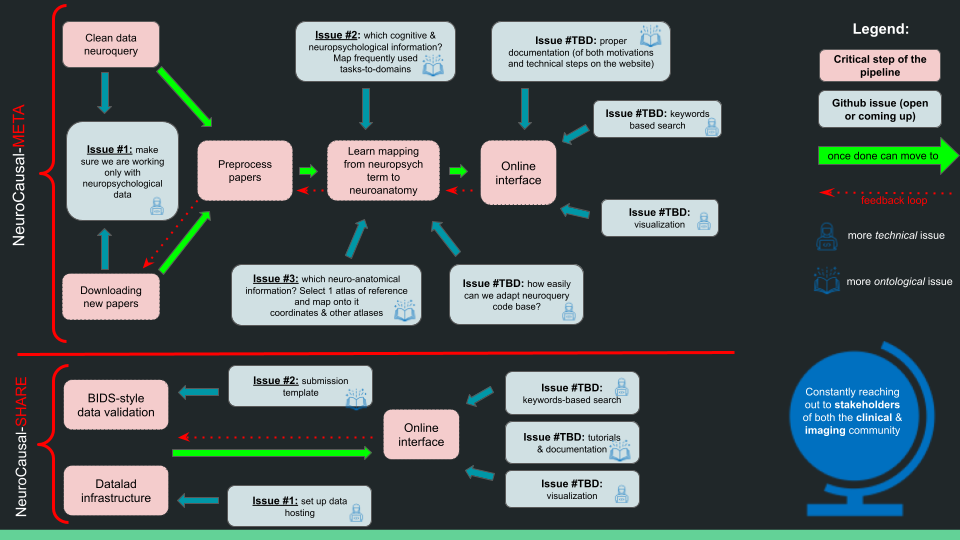
\includegraphics[width=0.5\textwidth]{NeuroCausal_BHproceeding.png}
	\caption{NeuroCausal: The future of neuropsychology, i.e. brain lesions-symptom mapping, will be transdiagnostic, open, and FAIR: we set out to provide the field with an open-source platform fostering storage, sharing, synthesis, and meta-analysis of clinical data.
}
	% Add a label to reference in text. Make it specific!
	\label{fig:NeuroCausal}
\end{figure}

\boldsymbol{Acknowledgments:} The authors would like to thank Eric Earl, Samuel Guay, Jerome Dockès, Bertrand Thirion, Jean Baptiste Poline, Yaroslav Halchenko, Sara El-Gebali and the whole Open Life Science team for their help and support.

\printbibliography

\end{document}